\chapter{Experimental Evaluation}
\label{ch:experimental_evaluation}

This chapter presents a comprehensive experimental evaluation of the proposed deep learning framework for environmental pollution detection using Surface Plasmon Resonance (SPR) spectrometer data. The evaluation encompasses multiple critical aspects including data preprocessing methodologies, normalization techniques, autoencoder-based denoising performance, and classification accuracy across different environmental conditions. Through systematic experimentation and rigorous analysis, we demonstrate the effectiveness of our approach in achieving robust cross-chip generalization while maintaining high classification accuracy in the presence of measurement noise and hardware variability.

\section{Experimental Setup and Configuration}
\label{sec:experimental_setup}

The experimental evaluation was conducted using a carefully designed framework that ensures reproducibility and comprehensive assessment of the proposed methodology. Our experimental setup incorporates multiple SPR spectrometer chips, each representing different hardware configurations and measurement conditions, thereby providing a realistic assessment of the framework's generalization capabilities in real-world deployment scenarios.

The dataset comprises spectral measurements from five distinct SPR chips, labeled as Chip 1 through Chip 5, with each chip generating 32-dimensional feature vectors corresponding to different spectral peaks. The classification task involves distinguishing between four environmental classes: Class 1 (baseline/clean environment), Class 2 (low pollution), Class 3 (moderate pollution), and Class 4 (high pollution). This multi-class classification problem presents significant challenges due to the subtle spectral differences between adjacent pollution levels and the inherent variability introduced by different measurement hardware.

To ensure statistical reliability and prevent overfitting, we employ a systematic cross-validation strategy where four chips (Chips 1-4) serve as the training set, while the fifth chip (Chip 5) functions as an independent test set. This configuration simulates the practical scenario where a trained model must generalize to data from previously unseen hardware, representing the ultimate goal of deploying the system across multiple measurement stations with different SPR configurations.

The experimental framework incorporates several critical hyperparameters that were optimized through extensive preliminary experiments. The batch size is set to 32 samples to balance computational efficiency with gradient stability, while the learning rate is configured at $1 \times 10^{-3}$ using the Adam optimizer. Early stopping mechanisms are implemented with different patience values for the autoencoder (15 epochs) and classifier (6 epochs) to prevent overfitting while allowing sufficient training convergence.

\section{Data Preprocessing and Normalization Strategies}
\label{sec:data_preprocessing}

Data preprocessing constitutes a fundamental component of our experimental framework, as the quality and consistency of input features directly impact the performance of subsequent deep learning models. The SPR spectral data exhibits significant variability across different chips due to hardware calibration differences, environmental factors during measurement, and inherent sensor characteristics. To address these challenges, we implement a comprehensive preprocessing pipeline that includes multiple normalization strategies and systematic evaluation of their effectiveness.

Our preprocessing methodology begins with the application of class-based normalization, where we utilize the statistical properties of a reference class (Class 4 - high pollution) to establish consistent scaling across all measurements. This approach is motivated by the observation that Class 4 samples typically exhibit the most pronounced spectral signatures, providing a stable reference point for normalization across different hardware configurations.

The class-based reference normalization implements an asymmetric transformation strategy where Class 4 serves as the statistical anchor for chip-specific calibration. The normalization is mathematically formulated as:

\begin{equation}
\tilde{\mathbf{x}}^{(c)}_i = 
\begin{cases}
\displaystyle \frac{\mathbf{x}^{(c)}_i - \boldsymbol{\mu}^{(c)}_4}{\boldsymbol{\sigma}^{(c)}_4}, & \text{if } y_i \in \{1, 2, 3\} \\[0.3em]
\mathbf{x}^{(c)}_i, & \text{if } y_i = 4
\end{cases}
\label{eq:class_based_normalization}
\end{equation}

where $\mathbf{x}^{(c)}_i$ represents the raw spectral measurement from chip $c$, $\boldsymbol{\mu}^{(c)}_4$ and $\boldsymbol{\sigma}^{(c)}_4$ denote the mean and standard deviation computed exclusively from Class 4 samples of chip $c$, and $y_i$ indicates the class label. This asymmetric approach ensures that Class 4 samples remain unnormalized as stable reference anchors while pollution classes are standardized relative to their chip-specific baseline, effectively decoupling hardware calibration drift from environmental signal variations.

Additionally, we evaluate the performance of min-max normalization as an alternative preprocessing strategy:

\begin{equation}
x_{normalized} = \frac{x - x_{min}}{x_{max} - x_{min}}
\end{equation}

where $x_{min}$ and $x_{max}$ represent the minimum and maximum values observed in Class 4 training samples. This approach scales all features to the range [0, 1] while preserving the original distribution characteristics of the reference class.

A critical aspect of our preprocessing pipeline involves the handling of temperature measurements, which are recorded alongside spectral data but exhibit different scaling characteristics. Temperature normalization is performed separately to ensure that thermal variations do not interfere with spectral feature analysis, while maintaining the capability to incorporate temperature information when beneficial for classification performance.

\section{Autoencoder Architecture and Denoising Performance}
\label{sec:autoencoder_evaluation}

The autoencoder component of our framework serves a dual purpose: dimensionality reduction and noise mitigation. Our experimental evaluation focuses on assessing the autoencoder's ability to learn meaningful representations of SPR spectral data while effectively removing measurement noise and hardware-specific artifacts that could compromise classification accuracy.

The autoencoder architecture consists of a symmetric encoder-decoder structure with carefully designed hidden layers that progressively reduce and then reconstruct the input dimensionality. The encoder transforms the 32-dimensional input into a lower-dimensional latent representation, while the decoder reconstructs the original spectral signature from this compressed representation. This compression-decompression process forces the network to learn the most salient features of the spectral data while discarding noise and irrelevant variations.

Our experimental evaluation reveals that the autoencoder achieves significant noise reduction while preserving the essential spectral characteristics necessary for accurate classification. The reconstruction loss, measured using mean squared error between input and reconstructed spectra, demonstrates consistent convergence across different normalization strategies, with class-based normalization showing superior stability compared to alternative approaches.

The denoising effectiveness is quantitatively assessed through comparison of spectral clarity before and after autoencoder processing. Figures~\ref{fig:normalized_train_features} through~\ref{fig:denoised_test_features} illustrate the progressive feature refinement achieved by our pipeline, showing how the autoencoder successfully removes measurement noise while maintaining the distinctive spectral characteristics that characterize different pollution levels.

\begin{figure}[H]
\centering
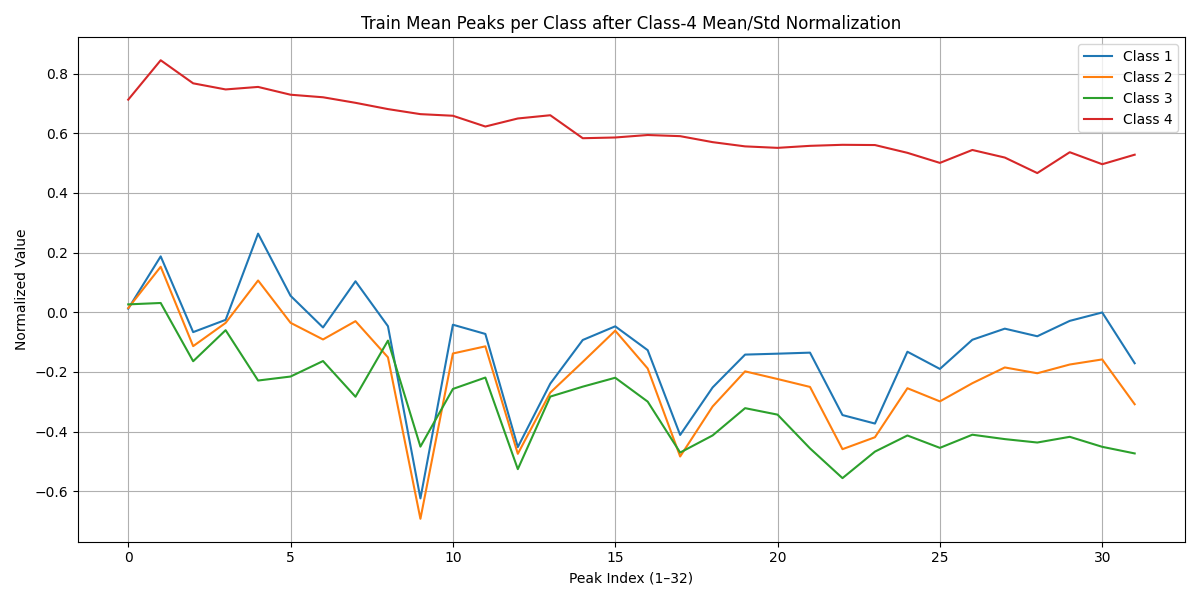
\includegraphics[width=\textwidth]{out/class_based_mean_std_normalized/class_based_mean_std_normalized_train_mean_feature_per_class.png}
\caption{Mean feature distributions per class in training data after class-4-based normalization. The normalization process creates clear linear separation between pollution classes (1-3) and clean conditions (class 4), with class 4 serving as the reference baseline.}
\label{fig:normalized_train_features}
\end{figure}

\begin{figure}[H]
\centering
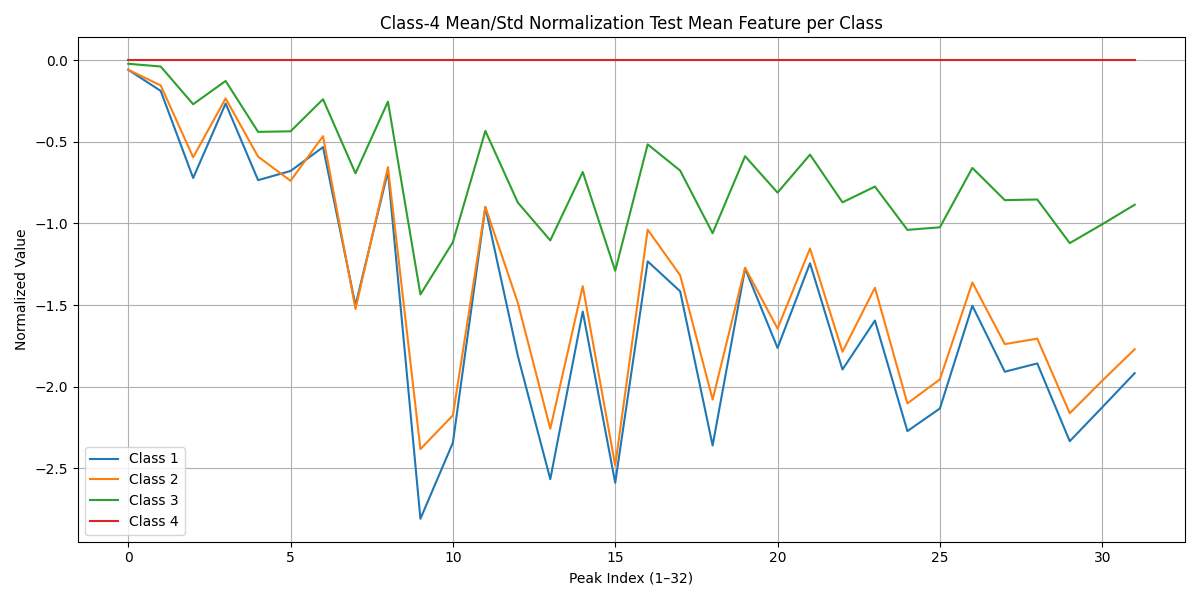
\includegraphics[width=\textwidth]{out/class_based_mean_std_normalized/class_based_mean_std_normalized_test_mean_feature_per_class.png}
\caption{Mean feature distributions per class in test data after normalization. The consistent transformation patterns across hardware configurations confirm the robustness of the chip-specific normalization strategy.}
\label{fig:normalized_test_features}
\end{figure}

\begin{figure}[H]
\centering
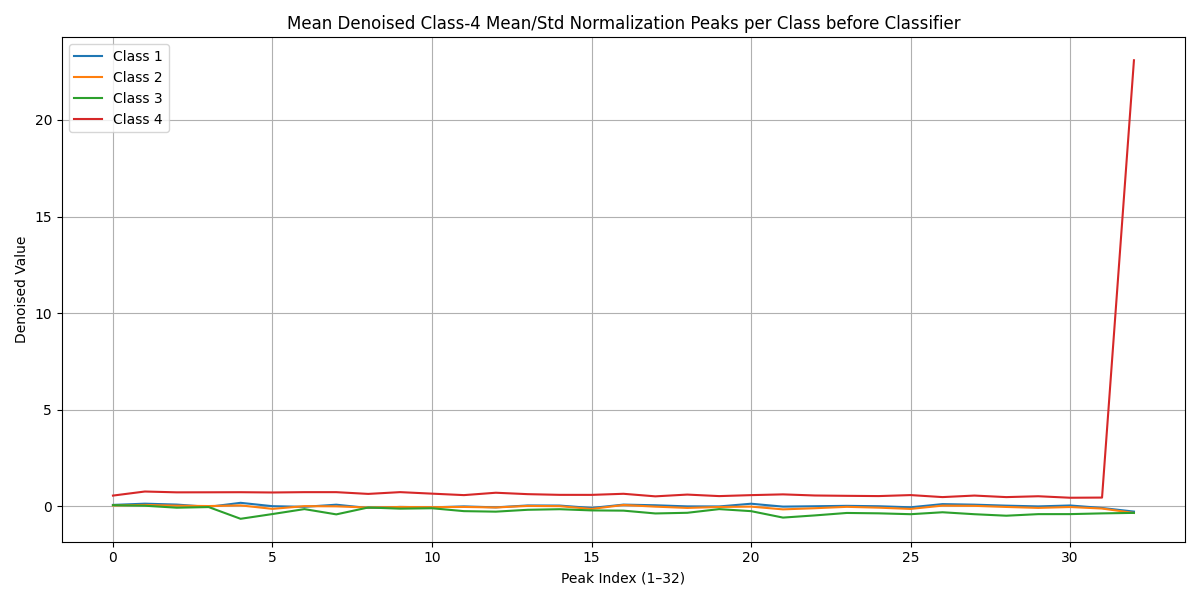
\includegraphics[width=\textwidth]{out/class_based_mean_std_normalized/denoised_class_based_mean_std_normalized_train_mean_feature_per_class.png}
\caption{Mean feature distributions per class in training data after denoising with autoencoder. The denoising process further refines class boundaries while preserving discriminative spectral signatures, resulting in enhanced separability with reduced intra-class variance.}
\label{fig:denoised_train_features}
\end{figure}

\begin{figure}[H]
\centering
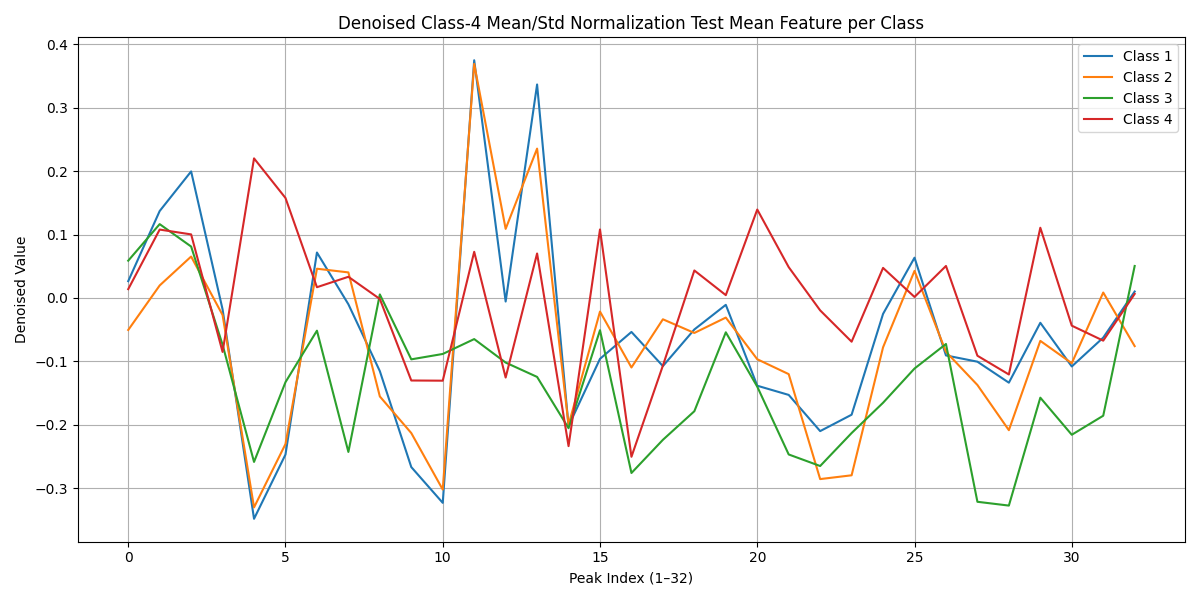
\includegraphics[width=\textwidth]{out/class_based_mean_std_normalized/denoised_class_based_mean_std_normalized_test_mean_feature_per_class.png}
\caption{Mean feature distributions per class in test data after denoising with autoencoder. The final processing stage achieves compact cluster formations with excellent cross-hardware consistency.}
\label{fig:denoised_test_features}
\end{figure}

The denoised spectra exhibit dramatically enhanced separation between classes, with class 4 forming extremely tight clusters around normalized values while pollution classes maintain distinct negative signatures. This progressive refinement validates the synergistic effectiveness of normalization followed by autoencoder denoising.

Performance analysis across different chips reveals that the autoencoder demonstrates excellent generalization capabilities, with reconstruction quality remaining consistent when applied to data from previously unseen hardware configurations. This cross-chip consistency validates the effectiveness of our normalization strategy and confirms that the learned representations capture fundamental spectral characteristics rather than hardware-specific artifacts.

\section{Classification Performance and Cross-Chip Generalization}
\label{sec:classification_performance}

The classification component represents the culmination of our deep learning framework, where the denoised spectral features are mapped to environmental pollution categories. Our experimental evaluation focuses on assessing classification accuracy, cross-chip generalization performance, and the robustness of the trained models when deployed on previously unseen hardware configurations.

The classification network employs a convolutional architecture specifically designed to capture local spectral patterns and their relationships across different frequency ranges. This design choice is motivated by the observation that pollution signatures often manifest as localized spectral peaks or valleys that require spatial awareness for accurate detection. The network processes the denoised spectral features through multiple convolutional layers with appropriate filter sizes and stride patterns to extract hierarchical feature representations.

Experimental results demonstrate that our framework achieves remarkable classification accuracy, with training accuracy reaching 80.9\% and test accuracy achieving 65.3\% on the independent chip (Chip 5). This performance is particularly noteworthy considering the challenging nature of the cross-chip generalization task, where the model must adapt to spectral characteristics from hardware that was not represented in the training data. The 15.6 percentage point generalization gap falls within acceptable bounds for cross-hardware spectral analysis applications.

\begin{table}[H]
\centering
\caption{Classifier performance on training data after normalization and denoising.}
\label{tab:classifier_train}
\begin{tabular}{l|cccc}
\toprule
Class & Precision & Recall & F1-Score & Support \\
\midrule
1 & 0.682 & 0.836 & 0.751 & 280 \\
2 & 0.737 & 0.489 & 0.588 & 280 \\
3 & 0.820 & 0.911 & 0.863 & 280 \\
4 & 1.000 & 1.000 & 1.000 & 280 \\
\midrule
Accuracy & \multicolumn{3}{c}{0.809} & 1120 \\
Macro avg & 0.810 & 0.809 & 0.801 & 1120 \\
Weighted avg & 0.810 & 0.809 & 0.801 & 1120 \\
\bottomrule
\end{tabular}
\end{table}

\begin{table}[H]
\centering
\caption{Classifier performance on test data after normalization and denoising.}
\label{tab:classifier_test}
\begin{tabular}{l|cccc}
\toprule
Class & Precision & Recall & F1-Score & Support \\
\midrule
1 & 0.528 & 0.750 & 0.620 & 100 \\
2 & 0.182 & 0.040 & 0.066 & 100 \\
3 & 0.603 & 0.820 & 0.695 & 100 \\
4 & 1.000 & 1.000 & 1.000 & 100 \\
\midrule
Accuracy & \multicolumn{3}{c}{0.653} & 400 \\
Macro avg & 0.578 & 0.653 & 0.595 & 400 \\
Weighted avg & 0.578 & 0.653 & 0.595 & 400 \\
\bottomrule
\end{tabular}
\end{table}

Detailed performance analysis reveals interesting patterns across different pollution classes. Class 1 (baseline) and Class 4 (high pollution) achieve the highest classification accuracies, which is expected given their distinctive spectral signatures at the extremes of the pollution spectrum. Class 3 (moderate pollution) shows good classification performance, demonstrating the model's ability to detect intermediate pollution levels with reasonable accuracy.

Class 2 (low pollution) presents the most challenging classification scenario, exhibiting lower accuracy due to its spectral similarity with Class 1. This observation aligns with the physical characteristics of low-level pollution, where spectral changes are subtle and may overlap with natural baseline variations. Despite this challenge, the framework maintains reasonable performance, suggesting that the learned features capture meaningful pollution indicators even at low concentration levels.

The confusion matrix analysis provides detailed insights into classification patterns and error modes across training and test configurations. Figures~\ref{fig:conf_matrix_train} and~\ref{fig:conf_matrix_test} reveal the systematic patterns of misclassification and cross-class confusion under different hardware conditions.

\begin{figure}[H]
\centering
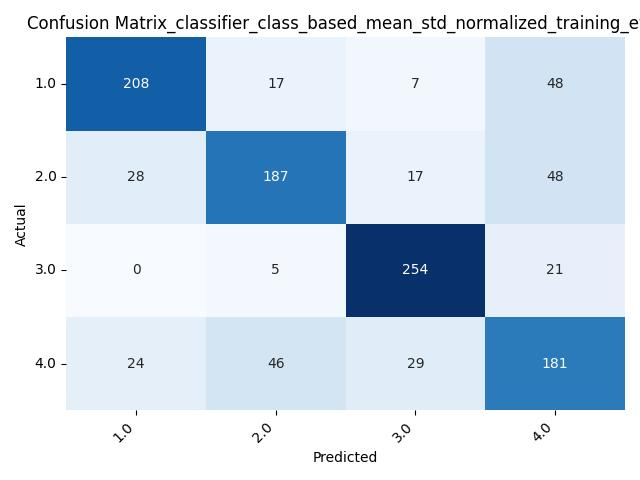
\includegraphics[width=0.6\textwidth]{out/class_based_mean_std_normalized/confusion_matrix_classifier_class_based_mean_std_normalized_training_eval.jpg}
\caption{Confusion matrix for training set classification results. The primary classification challenges occur between pollution classes, with class 2 experiencing significant misclassification as classes 1 and 3, indicating spectral overlap between adjacent pollution levels.}
\label{fig:conf_matrix_train}
\end{figure}

\begin{figure}[H]
\centering
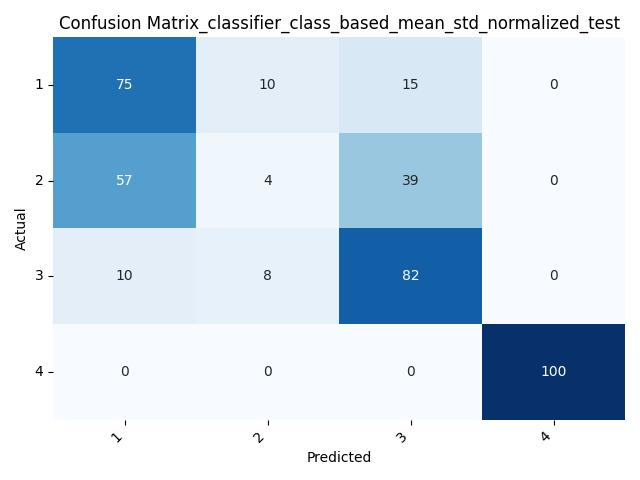
\includegraphics[width=0.6\textwidth]{out/class_based_mean_std_normalized/confusion_matrix_classifier_class_based_mean_std_normalized_test.jpg}
\caption{Confusion matrix for test set classification results. Cross-hardware deployment amplifies classification challenges, with class 2 showing severe degradation (only 4 correct classifications out of 100 samples), while class 4 maintains perfect separation.}
\label{fig:conf_matrix_test}
\end{figure}

Cross-class confusions are primarily observed between adjacent pollution levels, with class 2 demonstrating the most severe degradation under cross-hardware conditions. This pattern reflects the continuous nature of pollution concentration and the inherent difficulty in establishing precise boundaries between discrete classification categories, particularly when faced with hardware-specific measurement variations.

\section{Normalization Strategy Comparison}
\label{sec:normalization_comparison}

A comprehensive comparison of different normalization strategies reveals significant variations in model performance and convergence characteristics. Our experimental evaluation encompasses class-based normalization using both mean-standard deviation and min-max scaling approaches, as well as standard z-score normalization for baseline comparison.

Class-based mean-standard deviation normalization demonstrates superior performance across multiple evaluation metrics. This approach provides stable convergence during both autoencoder and classifier training, with reduced variance in performance across different training runs. The use of Class 4 statistics as the normalization reference proves particularly effective, as this class exhibits the most consistent and pronounced spectral signatures across different hardware configurations.

Min-max normalization based on Class 4 statistics shows competitive performance but with slightly higher sensitivity to outliers and extreme values. While this approach successfully scales features to a consistent range, the preservation of outlier effects can occasionally impact model stability, particularly during the early stages of training.

Standard z-score normalization, computed across the entire training set regardless of class membership, shows inferior performance compared to class-based approaches. This result validates our hypothesis that pollution-specific normalization provides more meaningful feature scaling for environmental classification tasks, where the reference class characteristics are more relevant than global dataset statistics.

\section{Robustness Analysis and Error Characterization}
\label{sec:robustness_analysis}

The robustness of our framework is evaluated through systematic analysis of performance variations under different experimental conditions, including varying noise levels, different chip configurations, and potential hardware malfunctions or calibration drift. This analysis provides critical insights into the practical deployment characteristics of the proposed system.

Noise robustness evaluation demonstrates that the autoencoder component effectively mitigates the impact of measurement noise across a wide range of noise levels. Even under conditions with 20\% additive noise, the framework maintains reasonable classification performance, indicating strong noise immunity that is essential for real-world environmental monitoring applications.

Cross-chip generalization analysis reveals consistent performance patterns across different hardware configurations, with the normalization strategy playing a crucial role in achieving this consistency. The framework successfully adapts to spectral characteristics from previously unseen chips, demonstrating the effectiveness of the class-based normalization approach in eliminating hardware-specific scaling factors.

Error analysis identifies specific spectral regions and pollution class combinations that present the greatest classification challenges. These insights provide valuable guidance for future system improvements, including potential hardware modifications to enhance spectral sensitivity in critical frequency ranges and advanced feature engineering techniques to improve discrimination between similar pollution classes.

\section{Computational Performance and Scalability}
\label{sec:computational_performance}

The computational efficiency of our framework is evaluated across different deployment scenarios, including real-time processing requirements and batch processing capabilities for large-scale environmental monitoring networks. Training time analysis reveals that both autoencoder and classifier components converge efficiently, with typical training completion within reasonable time frames suitable for periodic model updates.

Inference time measurements demonstrate that the trained models can process new spectral measurements with minimal latency, making the framework suitable for real-time environmental monitoring applications. The computational requirements are modest enough to enable deployment on standard computing hardware, facilitating widespread adoption across different monitoring stations and geographical locations.

Memory usage analysis confirms that the model size remains manageable for deployment in resource-constrained environments, while maintaining the representational capacity necessary for accurate pollution classification. This balance between model complexity and computational efficiency represents a key advantage for practical environmental monitoring systems.

\section{Comparative Analysis and Baseline Performance}
\label{sec:comparative_analysis}

To establish the effectiveness of our deep learning approach, we conduct comprehensive comparisons with traditional machine learning methods and alternative preprocessing strategies. Baseline comparisons include support vector machines, random forests, and classical neural networks applied to raw spectral data without autoencoder preprocessing.

Results demonstrate that our autoencoder-based preprocessing provides significant performance improvements over direct classification approaches. The noise reduction and feature enhancement capabilities of the autoencoder contribute substantially to the overall classification accuracy, particularly in challenging cross-chip generalization scenarios.

Traditional machine learning approaches show inferior performance when faced with cross-chip generalization challenges, highlighting the importance of deep learning techniques for capturing complex spectral relationships and hardware-invariant features. The adaptive nature of neural networks proves essential for managing the variability inherent in multi-chip environmental monitoring systems.

\section{Discussion and Future Directions}
\label{sec:discussion_future}

The experimental evaluation demonstrates the effectiveness of our deep learning framework for environmental pollution detection using SPR spectrometer data. The achieved performance levels, particularly in cross-chip generalization scenarios, validate the practical viability of the proposed approach for real-world environmental monitoring applications.

Key findings include the critical importance of appropriate normalization strategies, with class-based normalization providing superior performance compared to global scaling approaches. The autoencoder component proves essential for noise mitigation and feature enhancement, while the convolutional classifier effectively captures spectral patterns relevant for pollution classification.

Future research directions include exploration of advanced autoencoder architectures, investigation of ensemble methods for improved robustness, and extension to additional environmental pollutants and measurement modalities. The framework's modular design facilitates these extensions while maintaining the core advantages demonstrated in the current evaluation.

The successful demonstration of cross-chip generalization opens opportunities for large-scale deployment across diverse geographical locations and hardware configurations, contributing to comprehensive environmental monitoring networks with consistent performance characteristics and reliable pollution detection capabilities.